
\graphicspath{{Chapter2/Figs/}}

\setcounter{chapter}{5}
\chapter*{Capítulo 2.} 
\addcontentsline{toc}{chapter}{Capítulo 2}
\setcounter{figure}{0}
\setcounter{table}{0}
\setcounter{section}{0}

{\LARGE Estudios genómicos sobre la biogénesis de precursores de miARNs en plantas.}

\section{Introducción.}
En nuestro grupo se está estudiando la biogénesis de miARNs, específicamente como los precursores son reconocidos y procesados en plantas \citep{Bologna2013}.
La biogénesis de los miARNs depende del reconocimiento de claves estructurales ubicadas en los precursores de miARN \citep{pmid21554756,citeulike:8816489,Bologna11112012}.
Estos precursores tienen estructuras de tallo-burbuja características \citep{Jones-Rhoades2006}, que se cree que proporciona las claves para el procesamiento del mismo y la liberación de los ARN pequeños de 21 nt.

Los precursores de miARNs en plantas son muy variables en tamaño y forma \citep{Bologna2013,citeulike:8816489}.
Esa variabilidad se puede observar entre distintas familias de precursores, pero a veces también entre una misma familia de precursores en distintas especies (Figura \ref{fig:hairpin_distribution}).

\begin{figure}[htbp!] 
    \centering    
    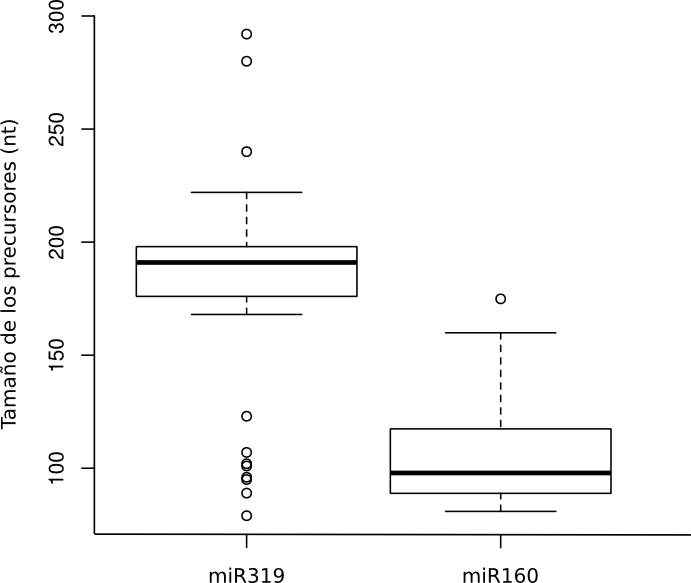
\includegraphics[width=.6\textwidth]{hairpin_distribution.png}
    \caption[Variación en el tamaño de precursores de miARNs de plantas]{
    \textbf{Variación en el tamaño de precursores de miARNs de plantas.} 
    Se muestra el tamaño (nt) de dos familias de precursores en distintas especies.}
    \label{fig:hairpin_distribution}
\end{figure}

Además, en las plantas, las mutaciones que impiden la biogénesis o actividad de los miARNs, tales como \textit{hyl1}, \textit{hen1} y \textit{ago1}, conducen al aumento en los niveles de los transcriptos de muchos de los genes blanco de miARNs (aproximadamente un 45\% de todos los blancos) \citep{Han2004,pmid12747833,pmid16889646,Allen2005207}.
Esto sugiere que el mecanismo que involucra el corte y degradación de los ARNm es un componente importante de la represión inducida por los miARNs en plantas \citep{Jones-Rhoades2006, Voinnet2009669}.

En particular, la biogénesis de los miARNs es un proceso clave porque determina la secuencia exacta de nucleótidos del ARN pequeño funcional.
En animales, los precursores poseen un tallo inferior de aproximadamente 11 pb, que se encuentra debajo de la posición donde DROSHA produce el corte.
Luego del primer corte llevado a cabo por DROSHA, el pre-miARN liberado está conformado por el dúplex miARN/miARN* y el loop terminal.
Estos pre-miARN son luego procesados a miARN maduros en el citoplasma mediante la interacción con la ribonucleasa Dicer.

Si bien en el caso de animales está claro cuáles elementos estructurales son reconocidos en los precursores durante su procesamiento, poco se sabía sobre el reconocimiento de los precursores de plantas por la maquinaria de procesamiento.

\subsection{Construcción de bibliotecas de SPARE para estudios genómicos de biogénesis de miARNs en plantas.}

En el marco de una colaboración con el grupo del Dr. Blake Meyers (Delaware,USA), el cual se especializa en secuenciación y análisis de ARN pequeños, nos propusimos entender cómo se procesan los precursores de miARNs en plantas. 
Colegas del laboratorio realizaron una estrategia para analizar sistemáticamente intermediarios de procesamiento de miARNs y caracterizar la biogénesis de los miARNs presentes en \textit{A. thaliana} mediante técnicas de secuenciación de alto rendimiento, utilizando los equipos de última generación disponibles en Delaware (USA).
Esta técnica desarrollada en el laboratorio se conoce como SPARE \citep{Schapire2013} (del inglés Specific Parallel Amplification of RNA Ends).
La estrategia utilizada a partir de los datos de bibliotecas de SPARE se muestra en la Figura \ref{fig:GR_fig1C}.

\begin{figure}[htbp!] 
    \centering    
    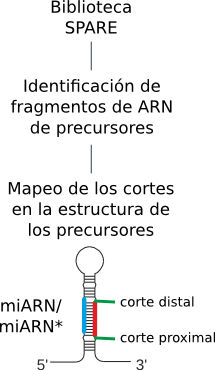
\includegraphics[width=.3\textwidth]{GR_fig1C.png}
    \caption[Esquema del procedimiento para analizar los datos de SPARE]{
        \textbf{Esquema del procedimiento para analizar los datos de SPARE.}
    }
    \label{fig:GR_fig1C}
\end{figure}

La técnica de SPARE, permite identificar los intermediarios de procesamiento de precursores de miARNs, y uniendo la información brindada por los diferentes fragmentos es posible dilucidar tanto la dirección, como el número de cortes requeridos para la biogénesis de cada miARN (Figura \ref{fig:SPARE_tecnica}).
Es decir que no sólo se puede detectar la dirección de procesamiento, sino que también la técnica permite identificar precursores que requieren más de dos cortes para liberar el miARN maduro.
Se utilizó esta técnica de SPARE para determinar el mecanismo de procesamiento cada uno de los precursores de \textit{A. thaliana}.

\begin{figure}[htbp!] 
	\centering    
	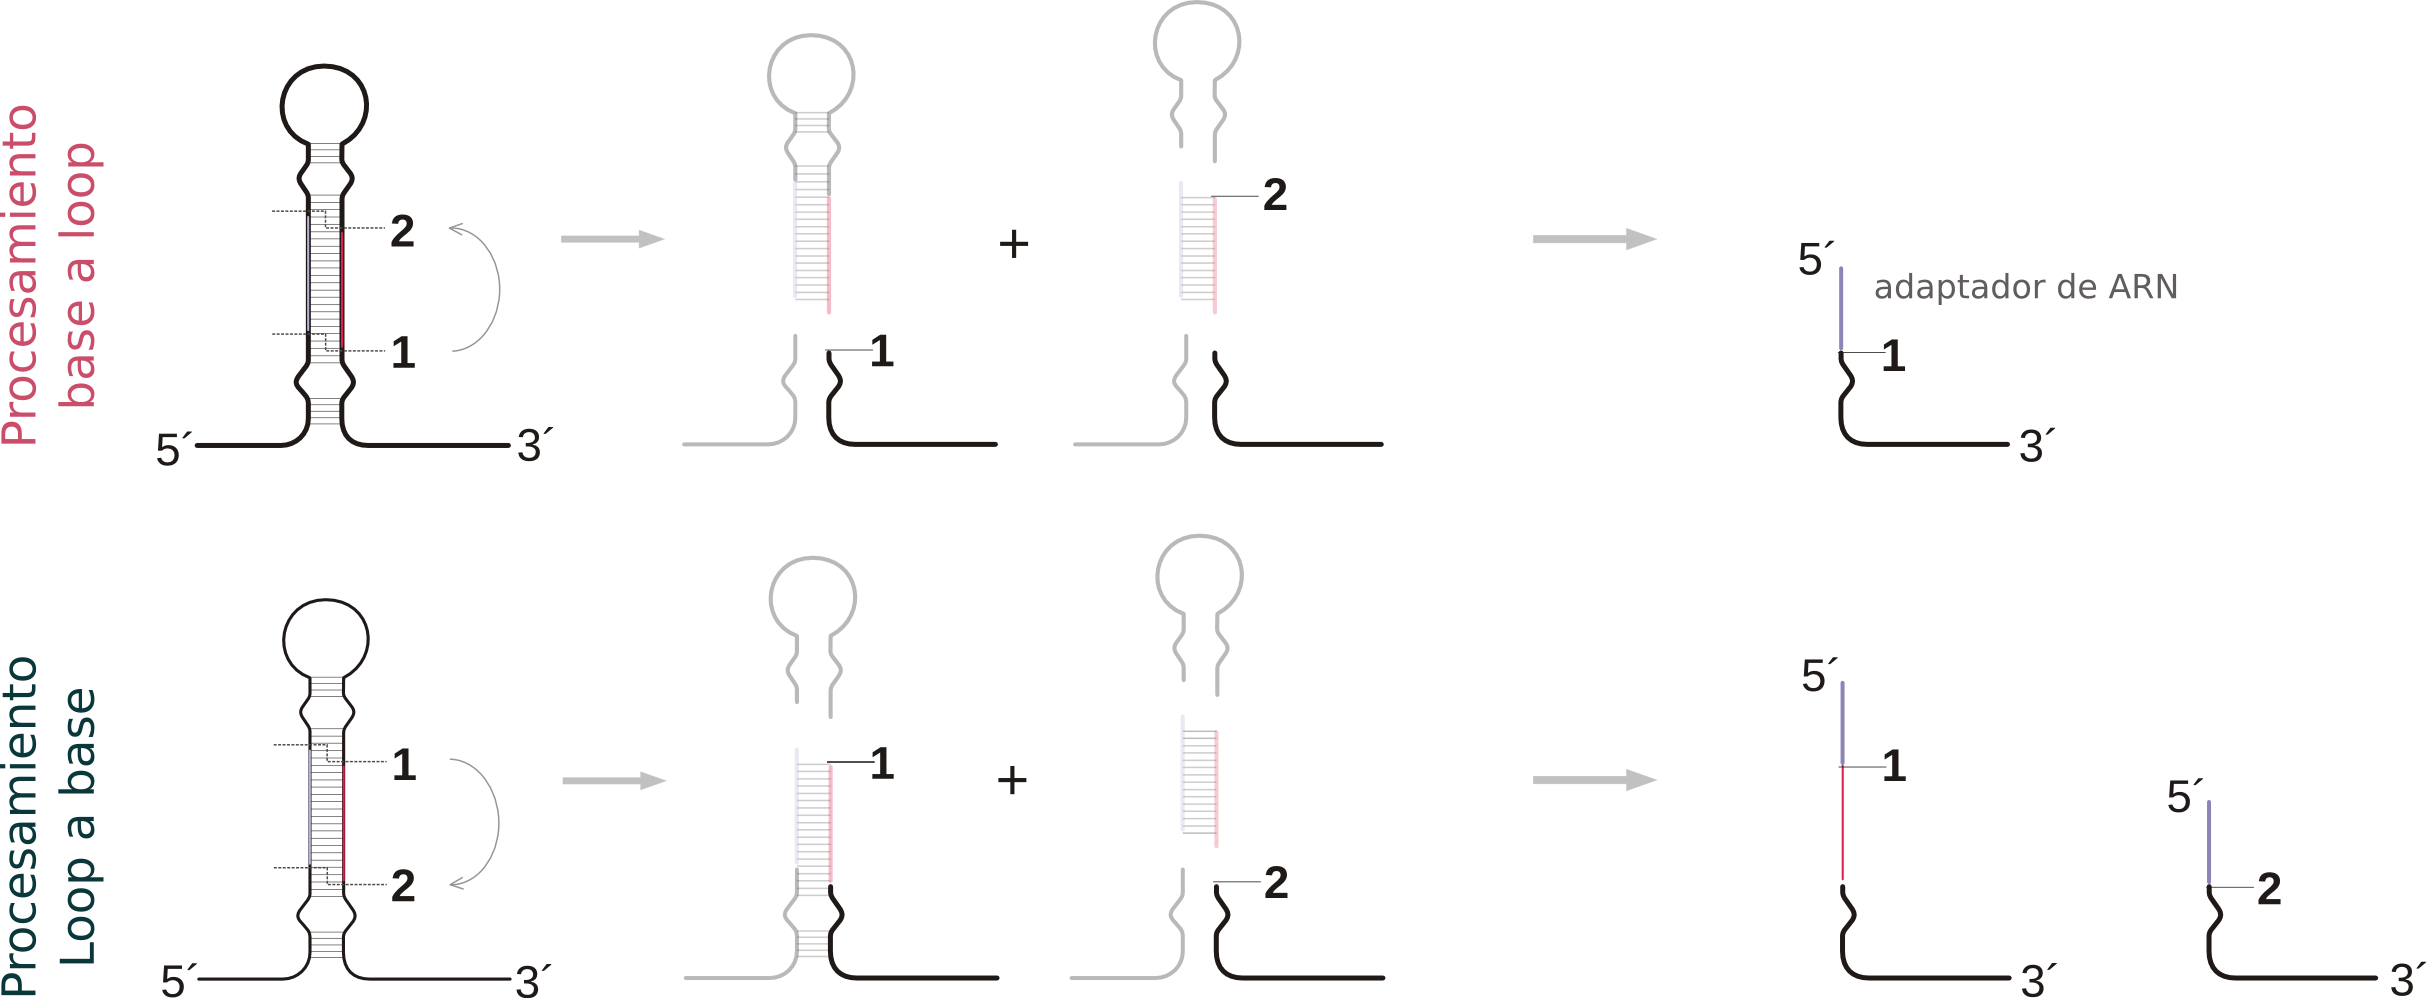
\includegraphics[width=1\textwidth]{SPARE_tecnica.png}
	\caption[Técnica de SPARE]{
        \textbf{Técnica de SPARE para diferenciar mecanismos de procesamiento de precursores.}
        Detalle donde se muestra a nivel molecular como la técnica permite diferenciar entre dos direcciones de procesamiento opuestas.
        Mediante la técnica se puede detectar un solo corte en los precursores procesados de base a loop.
        Mientras que para los precursores procesados de loop a base, la técnica permite detectar todos los cortes. 
    }
	 \label{fig:SPARE_tecnica}
\end{figure}

\subsection{Visualización de precursores que se procesan desde la base.}

En el caso de los precursores que se procesan de base a loop, el único corte que puede ser detectado es el corte proximal (Figura \ref{fig:GR_fig2A}).
En la Figura se puede ver el primer corte producido por DCL1 de los precursores del miR168a, miR172a y miR395b.
Las flechas indican la posición en que terminan los fragmentos secuenciados y el número representa el número de veces que ese fragmento se secuenció, y por lo tanto indica la abundancia de ese fragmento en la célula.
Se puede observar que este corte se da en una región de ARNdh ubicada a $\sim$15 nt desde el loop interno.
Por lo tanto se concluye que estos precursores de miARN tienen un tallo de ARNdh inferior a la región donde se ubica el propio miARN.
Puede verse que la gran mayoría de los cortes están ubicados en este sitio (Figura \ref{fig:GR_fig2A}).

\begin{figure}[htbp!] 
    \centering    
    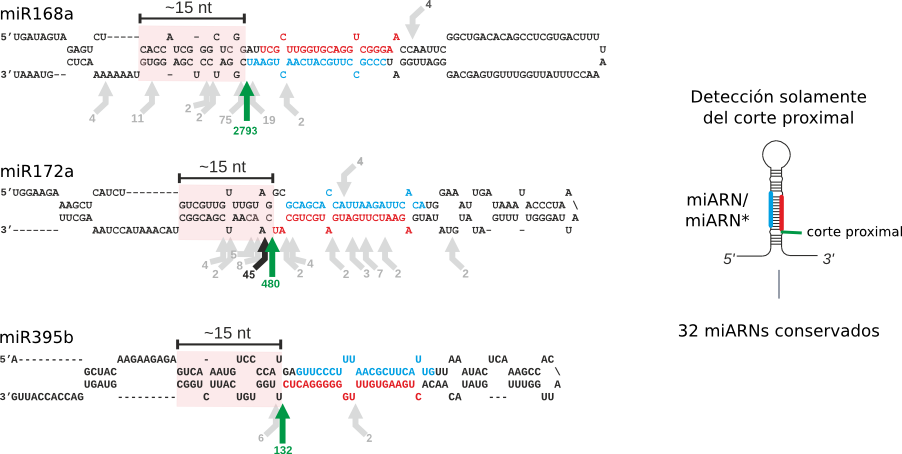
\includegraphics[width=.8\textwidth]{GR_fig2A.png}
    \caption[Identificación y caracterización de precursores de miARNs procesados de base a loop]{
    \textbf{Identificación y caracterización de precursores de miARNs procesados de base a loop.}
            Esquema donde se muestra la estructura secundaria del miR168a, miR172b y miR395b.
            Las flechas indican la posición y número de lecturas de los cortes del precursor identificado.
            Flechas en verde muestra el corte más abundante, que también coincide con al corte proximal del miARN/miARN*.
            Flechas en negro muestran otros cortes con al menos 5\% de abundancia del número total de cortes, mientras que otros cortes minoritarios se muestran con una flecha gris.
            En rosa se resalta el tallo de 15nt debajo del corte proximal.
            En celeste se resalta el ``loop'' interno. 
            El miARN se indica en color rojo y el miARN* en color azul.
            La imagen de la derecha muestra el patrón de corte típico detectado en la biblioteca de SPARE para estos precursores.}
    \label{fig:GR_fig2A}
\end{figure}

\subsection{Visualización de precursores que se procesan desde el loop.}

Para los precursores que se procesan de loop a base, la técnica de SPARE permite detectar tanto el corte distal como el proximal, que son los necesarios para liberar al miARN maduro (Figura \ref{fig:GR_fig4A}).
Además, en los precursores que necesitan más de dos cortes para liberar el miARN maduro, como la familia del miR319, los cuatro cortes pueden ser detectados por esta técnica.
En la figura se pueden ver los dos cortes por DCL1 de miembros de la familia del miR156 y del precursor del miR160a, que son procesados desde el loop a la base.

\begin{figure}[htbp!] 
    \centering    
    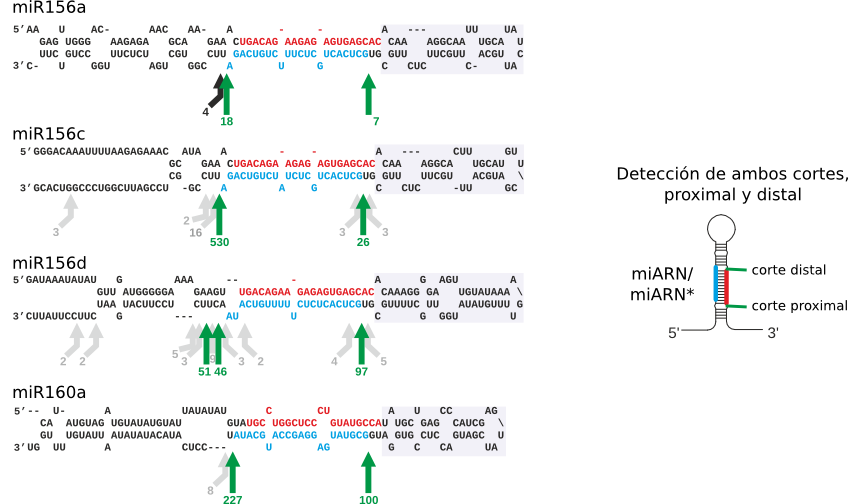
\includegraphics[width=.8\textwidth]{GR_fig4A.png}
    \caption[Identificación y caracterización de precursores de miARNs procesados de loop a base]{
    \textbf{Identificación y caracterización de precursores de miARNs procesados de loop a base.}
    Esquema donde se muestra la estructura secundaria del miR156a, miR156c, miR156d y miR160a.
    Las flechas indican la posición y número de lecturas de los cortes del precursor identificado.
    Flechas en verde muestra el corte más abundante, que también coincide con al corte proximal del miARN/miARN*.
    Flechas en negro muestran otros cortes con al menos 5\% de abundancia del número total de cortes, mientras que otros cortes minoritarios se muestran con una flecha gris.
    Con gris se resalta el tallo superior del miR156 y miR160. El miARN se indica en color rojo y el miARN* en color azul.
    La imagen de la derecha muestra el patrón de corte típico detectado en la biblioteca de SPARE para estos precursores.
}
    \label{fig:GR_fig4A}
\end{figure}


\section{Resultados y Discusión.}

\subsection{Desarrollo de herramienta para el análisis de intermediarios de procesamiento en \textit{A. thaliana}.}

\subsubsection{Análisis de las bibliotecas de SPARE y diseño de la herramienta.}

En una primera serie de experimentos, Nicolás Bologna y Arnaldo Schapire realizaron bibliotecas de SPARE en Col-0 y mutantes en \textit{fiery} para estudiar los intermediarios de procesamiento en \textit{A. thaliana}.
De esta técnica, se obtienen una gran cantidad de datos para cada biblioteca secuenciada y los primeros análisis se hicieron manualmente.

Por lo tanto se decidió en el laboratorio generar un protocolo bioinformático para el análisis de bibliotecas SPARE. 
Como material de partida, Belén Moro realizó nuevas bibliotecas de SPARE para precursores de \textit{A. thaliana} de plantas silvestres (Col-0) y en \textit{hyl1}, \textit{se} y \textit{fiery}.
El procesamiento y análisis de los datos se hizo a partir de los datos crudos y se detallan en Materiales y Métodos (ver sección \ref{sec:analisis_spare}).

Para ayudar a analizar estos datos complejos, desarrollamos una herramienta intuitiva para el análisis y visualización de los datos obtenidos por la técnica de SPARE.
Esto nos permite facilitar el análisis de la identificación de los intermediarios de procesamiento en de este tipo de bibliotecas.
Brevemente, en total se obtuvieron cerca de 150 millones de secuencias sumando todas las bibliotecas (Tabla \ref{SPARE_libraries}).
Los datos de la secuenciación son procesados y las secuencias correspondientes a fragmentos de precursores son agrupados y mapeados contra la totalidad de los precursores de miARN de \textit{A. thaliana}.

Esa información ya procesada es la que utilizamos en la herramienta para analizar y comparar los intermediarios de procesamiento para plantas silvestres y para las mutantes de procesamiento.

\begin{table}[]
    \centering
    \footnotesize
    \caption{Bibliotecas de SPARE}
    \label{SPARE_libraries}
    \begin{tabular}{llccc}
        \multicolumn{1}{c}{\cellcolor[HTML]{ECF4FF}\textbf{Bibliotecas}} & \multicolumn{1}{c}{\cellcolor[HTML]{ECF4FF}\textbf{Muestras}} & \cellcolor[HTML]{ECF4FF} \textbf{\begin{tabular}[c]{@{}c@{}}Secuencias\\ \\ totales\end{tabular}} & \cellcolor[HTML]{ECF4FF} \textbf{\begin{tabular}[c]{@{}c@{}}Secuencias\\ que mapean\\ los precursores\end{tabular}} & \cellcolor[HTML]{ECF4FF} \textbf{\begin{tabular}[c]{@{}c@{}}Secuencias únicas\\ que mapean\\ los precursores\end{tabular}} \\
        col\_2AB                                 & Col-0 réplica 1. Control de fiery y hyl1 & 13911694                                                                 & 80166                                                                                      & 308                                                                                               \\
        col\_3AB                                 & Col-0 réplica 2. Control de fiery y hyl1 & 16618008                                                                 & 126556                                                                                     & 426                                                                                               \\
        Col\_AD                                  & Col-0 réplica 1. Control de se           & 13758567                                                                 & 119368                                                                                     & 496                                                                                               \\
        Col\_BC                                  & Col-0 réplica 2. Control de se           & 14648459                                                                 & 241973                                                                                     & 553                                                                                               \\
        FIERY\_1AB                               & fiery réplica 1                          & 9832923                                                                  & 470789                                                                                     & 1655                                                                                              \\
        FIERY\_4                                 & fiery réplica 2                          & 23529725                                                                 & 821562                                                                                     & 1752                                                                                              \\
        HYL\_1                                   & hyl1 réplica 1                           & 10171629                                                                 & 45653                                                                                      & 316                                                                                               \\
        HYL\_2                                   & hyl1 réplica 2                           & 8864406                                                                  & 35860                                                                                      & 320                                                                                               \\
        SE\_BD                                   & se réplica 1                             & 15291993                                                                 & 299513                                                                                     & 639                                                                                               \\
        SE\_CE                                   & se réplica 1                             & 25296809                                                                 & 510438                                                                                     & 693                                                                                              
    \end{tabular}
\end{table}

La herramienta diseñada permite seleccionar un precursor en particular y luego seleccionar una o varias mutantes y controles que se quieren analizar.
Además, la herramienta permite modificar otros parámetros como la longitud y abundancia de los fragmentos secuenciados a considerar.

\subsubsection{Precursores procesados desde la base.}
Primero vemos la salida de la herramienta para el precursor del  miR165a, analizando distintas mutantes de procesamiento al mismo tiempo (Figura \ref{fig:miR165a_SPARE}).
La posición final del dúplex miARN/miARN* fue considerada como la posición 0, y las posiciones positivas son bases hacia (hacia el loop) arriba del dúplex mientras que las posiciones negativas son bases hacia abajo del dúplex.
Los fragmentos se muestran en forma porcentual tomando cada biblioteca de forma independiente y en distintos colores se representan las distintas bibliotecas.
Además, se muestra una tabla con los valores absolutos de cada fragmento y con flechas verdes se marcan las posiciones con los fragmentos de mayor abundancia en promedio de todas las bibliotecas (Figura \ref{fig:miR165a_SPARE}).
 
En esta figura se muestra un precursor que es procesado con un mecanismo corto de base a loop, donde según se muestra en la Figura \ref{fig:SPARE_tecnica}, los fragmentos detectados corresponden únicamente al primer corte por DCL1 (Figura \ref{fig:miR165a_SPARE}).
Se pueden observar también cortes en las posiciones $\pm 2$ con respecto a las esperadas por actividad ``sloopy'' (poco rigurosa) de DCL1 \citep{pmid17989254}.
Además se observan en la posición -5, que aparecen fragmentos en todas las bibliotecas aunque en muy baja abundancia (Figura \ref{fig:miR165a_SPARE}).
Por el momento, no hay una clara explicación para el origen mecanístico de estos cortes, pero muestra la utilidad de la herramienta para poder fácilmente visualizar e identificar elementos comunes e inesperados en distintas bibliotecas.


\begin{landscape}
    \begin{figure}[htbp!] 
        \centering    
        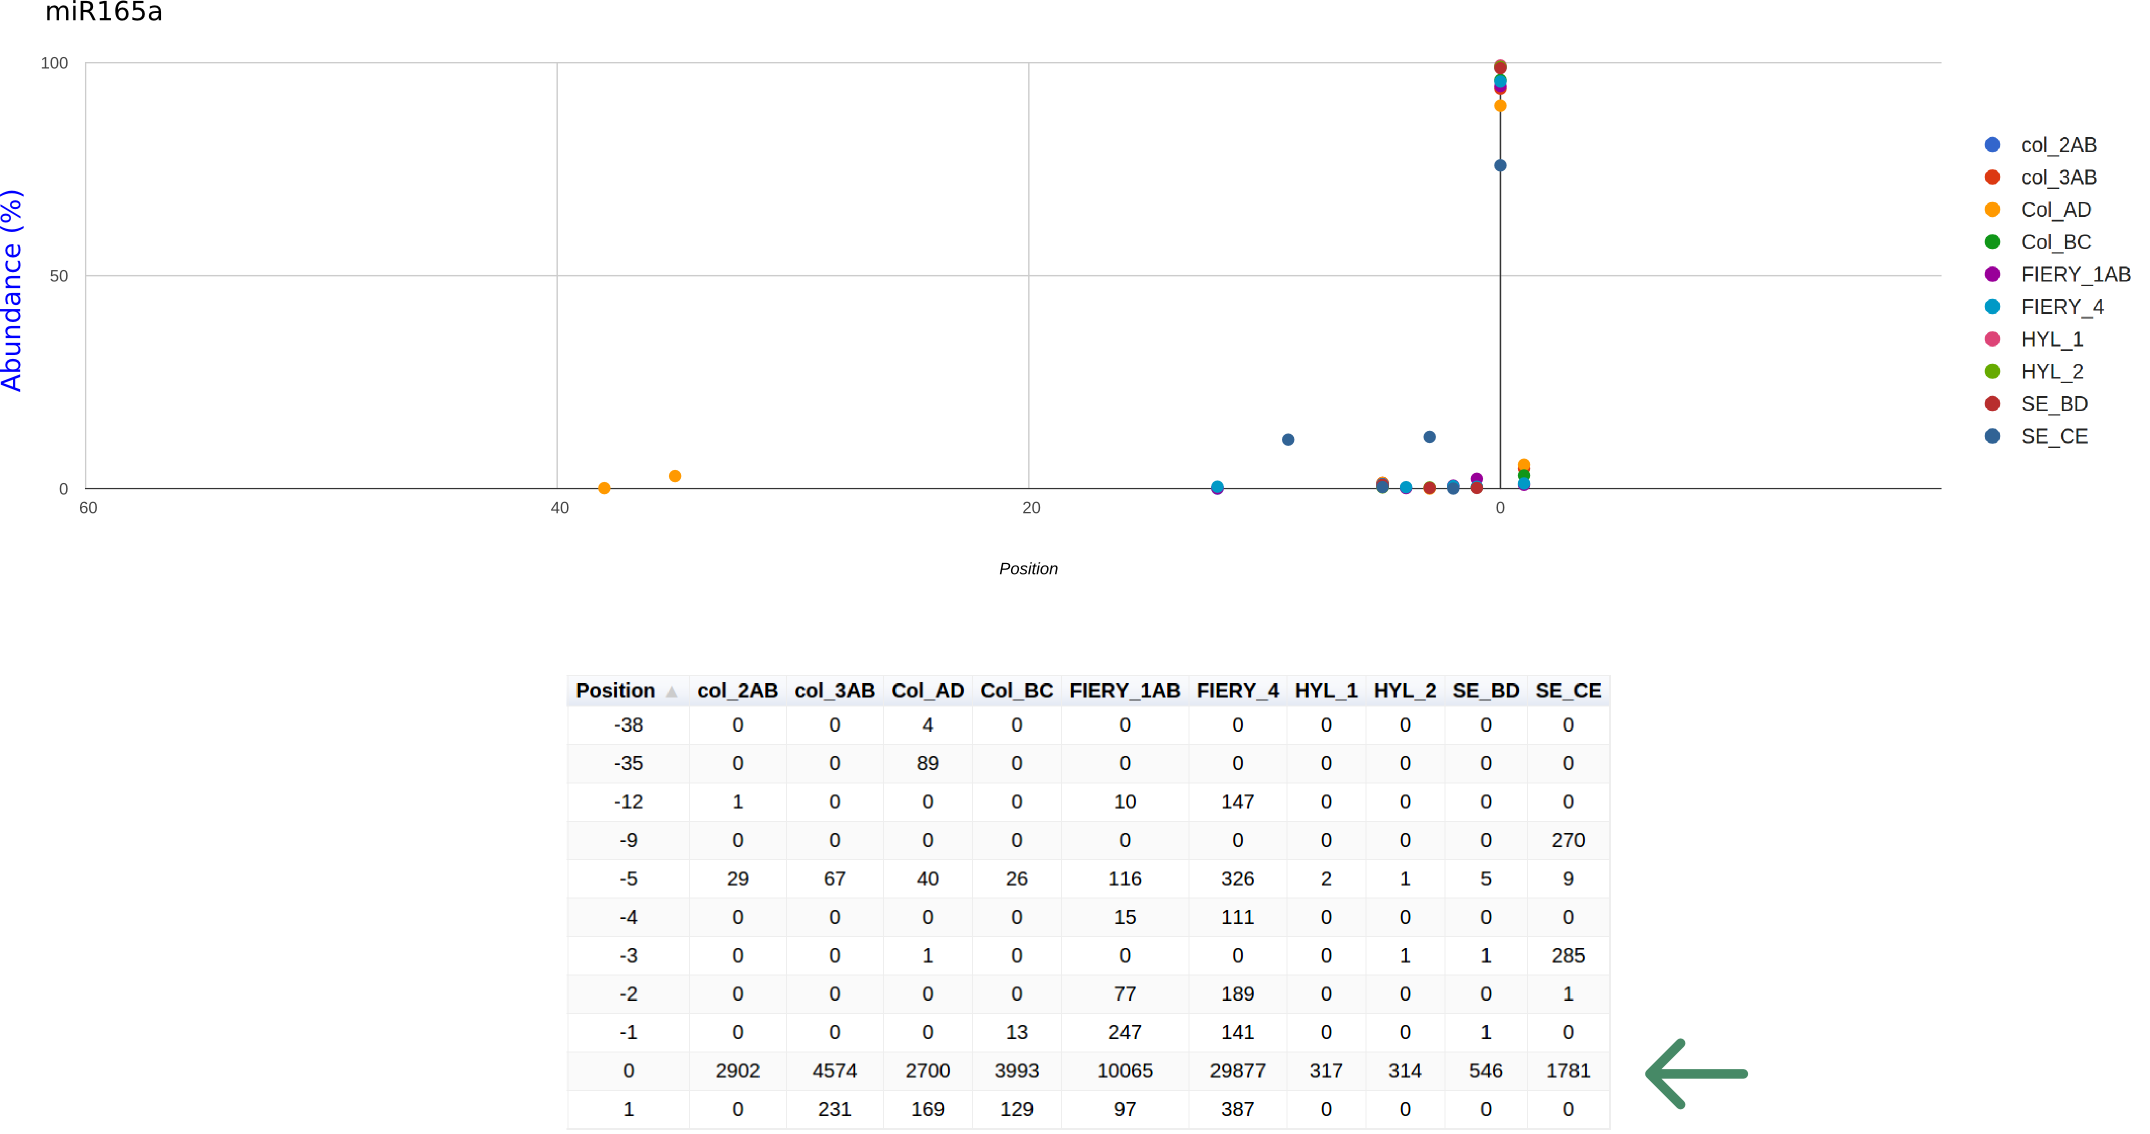
\includegraphics[width=1.4\textwidth]{miR165a_SPARE.png}
        \caption[Captura de pantalla de la herramienta de SPARE para el miR165a]{
        \textbf{Captura de pantalla de la herramienta de SPARE para el miR165a.}
        Porcentaje de fragmentos del precursor (abundancia relativa de los fragmentos en esa posición dividido la abundancia total de los fragmentos en el precursor).
        La posición final del dúplex miARN/miARN* fue considerada como la posición 0.
        La tabla muestra los valores absolutos de cada fragmento.
        Las flechas verdes marcan las posiciones del precursor con los fragmentos de mayor abundancia. 
        }
         \label{fig:miR165a_SPARE}
    \end{figure}
\end{landscape}

\subsubsection{Precursores procesados desde el loop.}

Para el caso de los precursores cortos de loop a base, los fragmentos del corte por DCL1 detectados, pueden ser más de uno según muestra la técnica de SPARE (Figura \ref{fig:SPARE_tecnica}).
Lo mismo sucede con los precursores de loop a base que son cortados más de dos veces por DCL1.
Para ilustrar esto, mostramos  el caso del miR159, que al igual que todos los precursores que son procesados secuenciales de loop a base, los cuatros fragmentos más abundantes corresponden a los cuatro cortes realizados por DCL1 que son requeridos para procesar este precursor (Figura \ref{fig:miR159b_SPARE}).
El primer corte se da en la posición 71, que de los cuatros cortes es el que tiene fragmentos menos abundantes, y luego DCL1 corta a 21 nucleótidos liberando otros ARN pequeños.
Luego se pueden observar los fragmentos correspondientes al tercer corte (posición 21) y cuarto corte (posición 0), que son los necesarios para liberar el miARN maduro (Figura \ref{fig:miR159b_SPARE}).
En este caso se pueden ver otros fragmentos, aunque nunca son tan abundantes como los correspondientes a los cortes por DCL1.
Por cuestiones de simplicidad, en la tabla solo se muestra los fragmentos con mayor abundancia en promedio de todas las bibliotecas.
Estos otros cortes posiblemente sean el resultado del corte improductivo del precursor por ribonucleasas y quizás sean parte de un proceso de degradación de los precursores.
Los orígenes de estos fragmentos del precursor están en estudio en el laboratorio.
El análisis de estas nuevas bibliotecas también permitió aumentar el número de precursores de miARNs de Arabidopsis caracterizados.

\begin{landscape}
    \begin{figure}[htbp!] 
        \centering    
        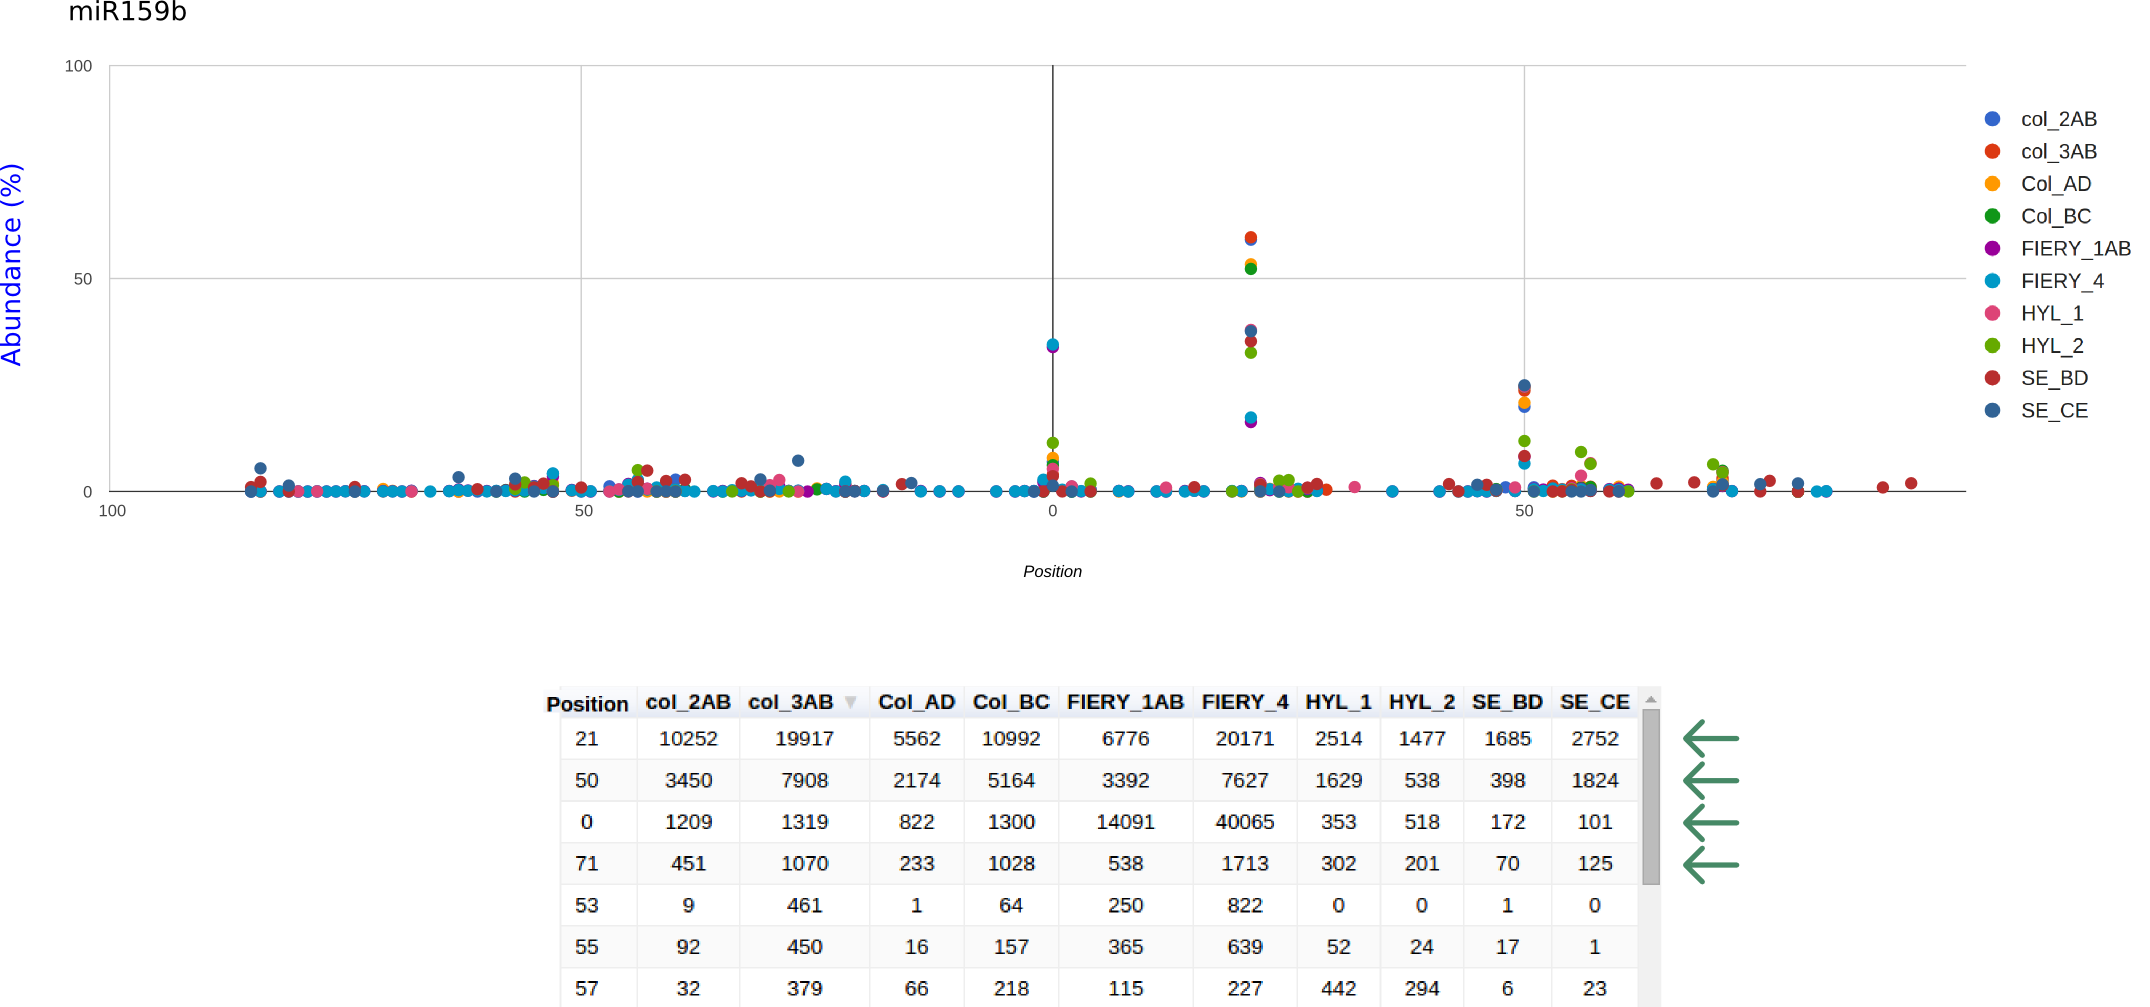
\includegraphics[width=1.4\textwidth]{miR159b_SPARE.png}
		\caption[Captura de pantalla de la herramienta de SPARE para el miR159b]{
        \textbf{Captura de pantalla de la herramienta de SPARE para el miR159b.}
        Porcentaje de fragmentos del precursor (abundancia relativa de los fragmentos en esa posición dividido la abundancia total de los fragmentos en el precursor).
        La posición final del dúplex miARN/miARN* fue considerada como la posición 0.
        La tabla muestra los valores absolutos de cada fragmento.
        Por cuestiones de simplicidad, solo se muestran en la tabla los fragmentos con mayor abundancia en promedio de todas las bibliotecas.
        Las flechas verdes marcan las posiciones del precursor con los fragmentos de mayor abundancia.
        }
		\label{fig:miR159b_SPARE}
    \end{figure}
\end{landscape}


\subsection{Análisis estructural de precursores de miARNs en plantas.}

Una vez que se pudo clasificar a los precursores de acuerdo a su tipo de procesamiento, ya sea desde el loop o desde la base, y sea con dos o mas cortes de DCL1, decidimos ver si había diferencias estructurales para cada grupo.
Los datos para este primer análisis fueron el SPARE realizado sobre las plantas silvestres y mutantes \textit{fiery}.

Primeramente, obtuvimos las estructuras secundarias para cada precursor  utilizando el programa Mfold\citep{pmid12824337} (Ver Materiales y Métodos sección \ref{sec:estruc_sec}) realizamos un análisis estructural conjunto de los precursores correspondientes a los dos mecanismos de procesamiento, los que se procesan en dirección base a loop (Figura \ref{fig:GR_fig2C}) y los que se procesan loop a base (Figura \ref{fig:GR_fig4C}).
Definimos a una coincidencia en cada posición con un 0, mientras que ``bulges'' y ``mismatches'' los consideramos como 1.
El lado proximal del dúplex miARN/miARN* fue definido como la posición +1 y analizamos desde la posición -25 a la posición +40 (Figura \ref{fig:GR_fig2C} y \ref{fig:GR_fig4C}). 

\subsubsection{Estructuras secundarias de precursores procesados desde la base.}

El análisis de los precursores que se procesan de base a loop mostró que todos ellos tienen un claro tallo inferior de 15 nt de largo (Figura \ref{fig:GR_fig2C}).
Este tallo se pudo observar tanto para los precursores validados experimentalmente en esta parte del trabajo, como para todos los precursores conservados que se procesan desde la base (Figura \ref{fig:GR_fig2C} en violeta).
También, pudimos observar que las bases inmediatamente debajo del dúplex miARN/miARN* (posición -2 y -1) tienden a estar desapareadas (Figura \ref{fig:GR_fig2C}).
Además, las posiciones -3 y -4 y las 3 últimas posiciones del tallo inferior (-13,-14 y -15) están apareadas casi siempre (Figura \ref{fig:GR_fig2C}).
En general, nuestros resultados muestran que los precursores procesados en una dirección base a loop son más uniformes de lo que se pensaba previamente.

\begin{figure}[htbp!] 
    \centering    
    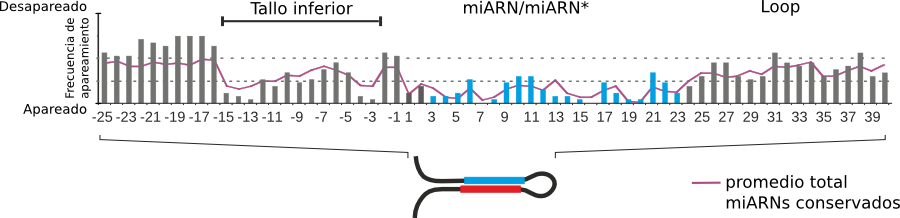
\includegraphics[width=1\textwidth]{GR_fig2C.png}
    \caption[Estructura secundaria de precursores de base a loop]{
    \textbf{Estructura secundaria de precursores detectados que se procesan en dirección base a loop.}
    Los matches en cada posición los consideramos como 0, mientras que ``bulges'' y ``mismatches'' fueron considerados como 1.
    La estructura secundaria considerando todos los miARNs conservados se indica con color violeta.
    }
    \label{fig:GR_fig2C}
\end{figure}

\subsubsection{Estructuras secundarias de precursores procesados desde el loop.}
Con la excepción de dos miARNs (miR396a y miR162b) estos precursores procesados desde el loop, no tienen una estructura obvia debajo del dúplex miARN/miARN* (Figura \ref{fig:GR_fig4C}).
En cambio, estos precursores tienen una región terminal estructurada (Figura \ref{fig:GR_fig4C}), que tiene un tamaño homogéneo de ~42nt que incluye un loop corto en contraste con la misma región en los precursores que se procesan de base a loop donde es más variable (Figura \ref{fig:GR_fig2C} y \ref{fig:GR_fig4C}). 

\begin{figure}[htbp!] 
    \centering    
    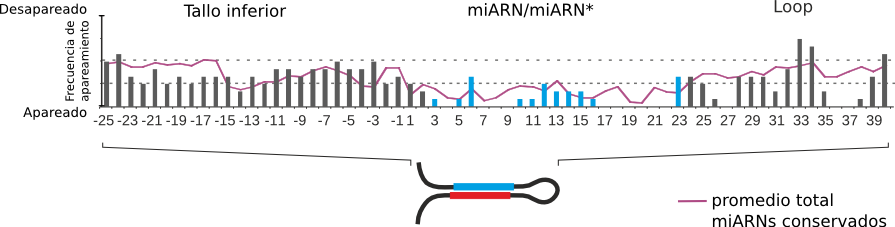
\includegraphics[width=1\textwidth]{GR_fig4C.png}
    \caption[Estructura secundaria de precursores de loop a base]{
   \textbf{ Estructura secundaria de precursores detectados que se procesan en dirección loop a base.}
    Los matches en cada posición los consideramos como 0, mientras que ``bulges'' y ``mismatches'' fueron considerados como 1.}
    \label{fig:GR_fig4C}
\end{figure}


\section{Conclusiones.}

En esta segunda parte del proyecto de Tesis presentamos una estrategia y para el análisis sistemático de las bibliotecas de SPARE y la identificación de la biogénesis de precursores de miARNs desde un punto de vista genómico.
Utilizando esta técnica encontramos que los miARNs son procesados por cuatro mecanismos, dependientes de la dirección secuencial de la maquinaria de procesamiento y del número de cortes requeridos para liberar el miARN (Figura \ref{fig:mecanismos}).

\begin{figure}[htbp!] 
    \centering    
    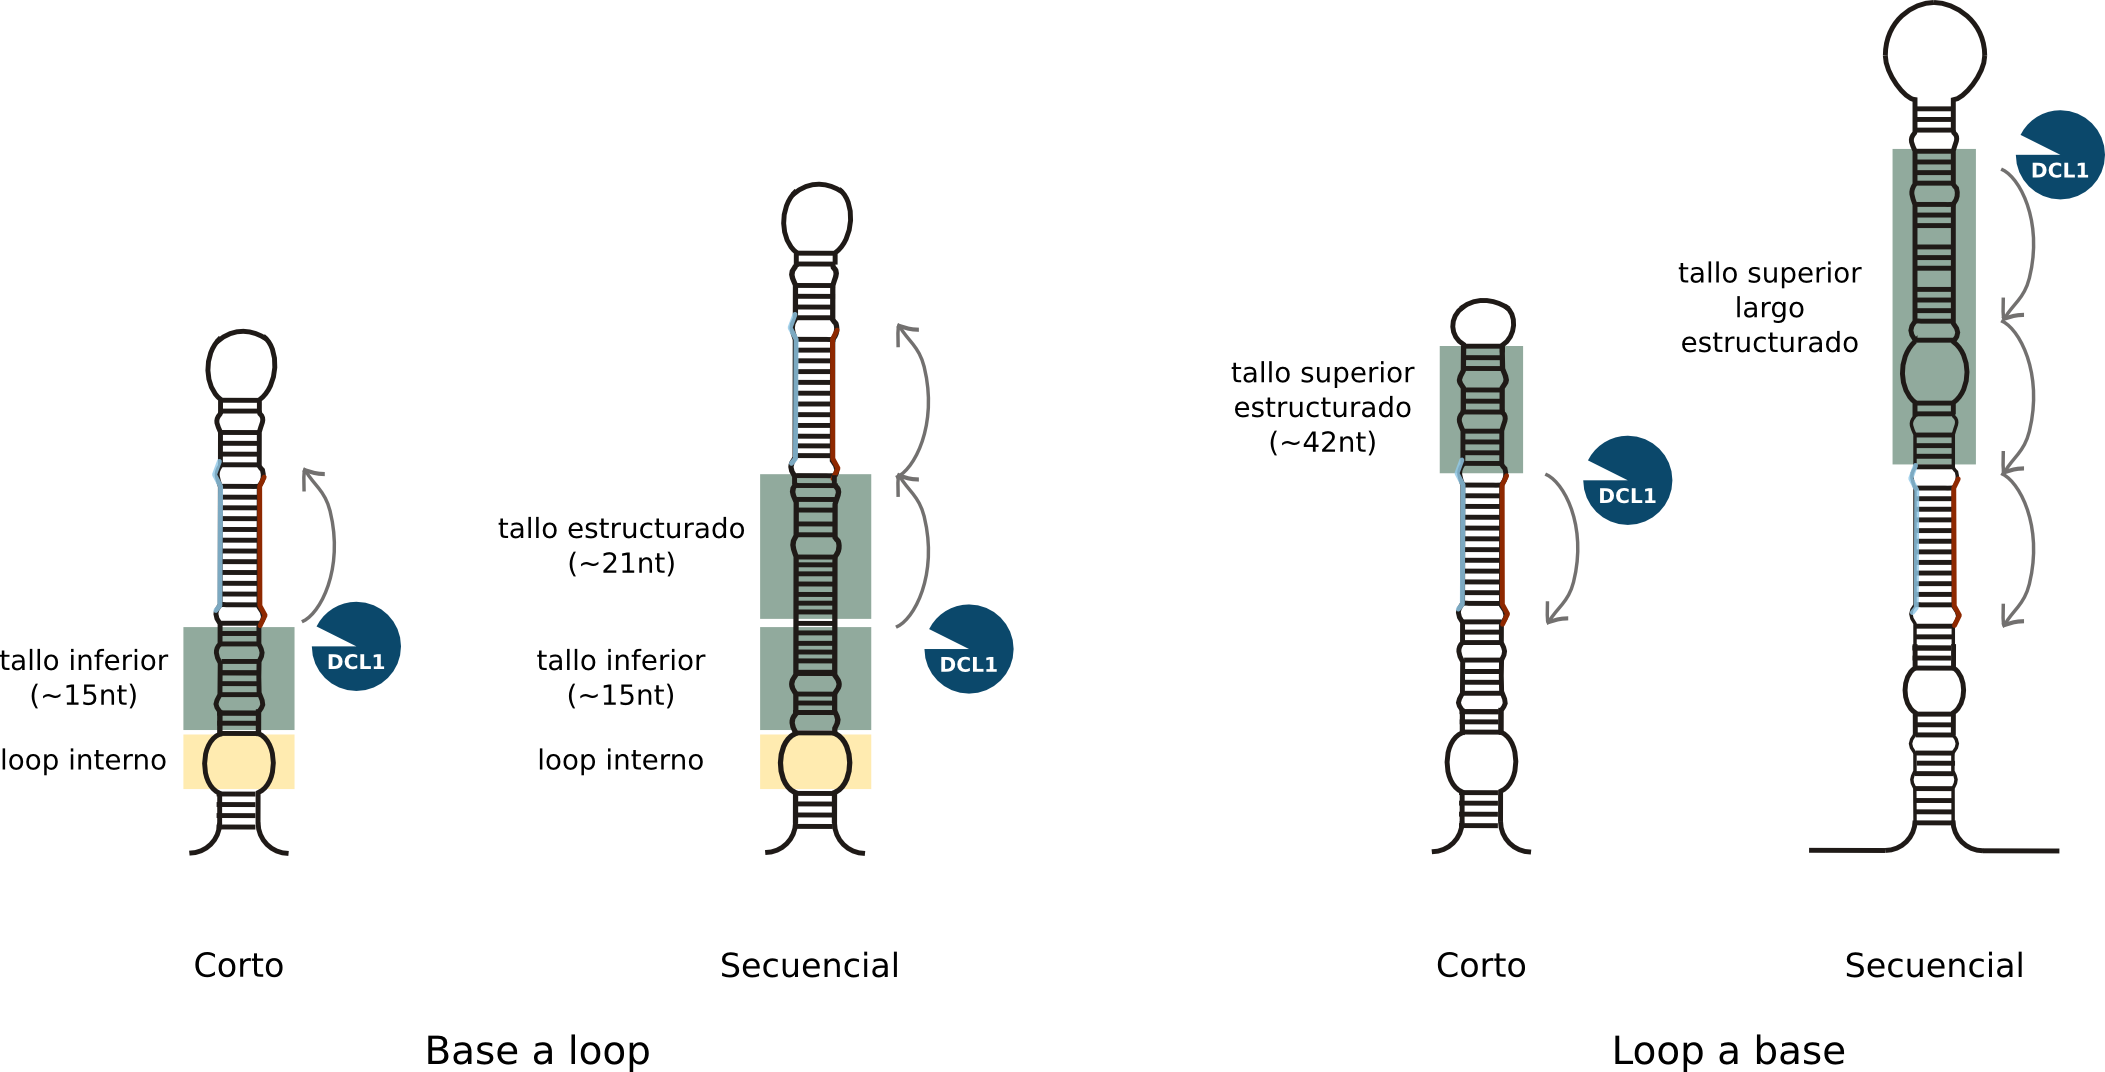
\includegraphics[width=1\textwidth]{mecanismos.png}
    \caption[Mecanismos de procesamiento]{
    \textbf{Distintos mecanismos de procesamientos de miARNs en plantas}
    A la izquierda se muestra los precursores que son procesado de base a loop.
    A la derecha se muestra los precursores que son procesado de loop a base.
    En ambos casos se muestran los precursores cortos y los secuenciales.
    Se identifica en azul el corte por DCL y con flechas la dirección de procesamiento.
        }
    \label{fig:mecanismos}
\end{figure}

La clasificación de los precursores, teniendo en cuenta los mecanismos de procesamiento y el análisis consiguiente para cada grupo, reveló determinantes estructurales específicos para cada grupo.

Integrando los resultados que se muestran en la introducción junto a los resultados obtenidos en esta Tesis, se pudo demostrar que los precursores de miARNs en plantas se pueden agrupar por cuatro mecanismos de procesamiento con distintas características (Figura \ref{fig:mecanismos}).

\begin{itemize}
    \item En los precursores con un mecanismo \textbf{corto de base a loop}, un loop interno seguido por un tallo inferior de $\sim$15nt especifica la posición del primer corte.
        Esta estructura se encuentra en la mayoría de familias de miARNs \citep{Mateos2010,pmid20015653,pmid20015654}.
        A pesar de que el tallo puede contener bulges, la transición de un loop interno (simple hebra) al tallo inferior es bastante marcada, y tres pares de bases apareadas generalmente definen el comienzo del tallo inferior del precursor \citep{Bologna2013}.
        El segundo corte procede a una distancia fija de $\sim$21 nt desde la posición del primer corte.
    \item En los precursores con un mecanismo \textbf{secuencial de base a loop} (ej: familia del miR169), el primer corte procede como en los cortos de base a loop, pero luego son necesario dos cortes más para liberar el miARN, generando en el proceso niveles bajos de RNA pequeños adicionales \citep{Bologna2013}.
    \item En los precursores con un mecanismo \textbf{cortos de loop a base} (ej: familia del miR156 y miR160), el procesamiento es guiado por un tallo superior, y son necesarios dos cortes para liberar el miARN maduro.
        La región terminal de estos precursores tienen una largo conservado de $\sim$42 donde incluye un loop pequeño \citep{Bologna2013}.
    \item En los precursores con un mecanismo \textbf{secuencial de loop a base} (ej: familia del miR319 y miR159), cuatro cortes secuenciales por DCL1 son los encargados de procesar los precursores de miARNs.
        En general muestran un tallo largo superior, del cual otros ARNs pequeños son generados \citep{pmid19850910,Bologna2009,Bologna2013}
\end{itemize}



Estos resultados fueron publicado en la revista Genome Research \citep{Bologna2013}.
Los resultados ofrecen una explicación para la diversidad estructural de los genes de precursores de miARN en plantas y nuevas perspectivas hacia la comprensión de la biogénesis de los ARNs pequeños \citep{Bologna2013}.

Y con esto, pudimos encontrar determinantes estructurales distintos para precursores que se procesados desde la base y precursores procesados desde el loop. 
